\documentclass[Main]{subfiles}
\begin{document}

\chapter{Design}

\section{System oversigt}

Til styring af drone, skal der laves en sender og modtager.

\begin{figure}[H]
\centering
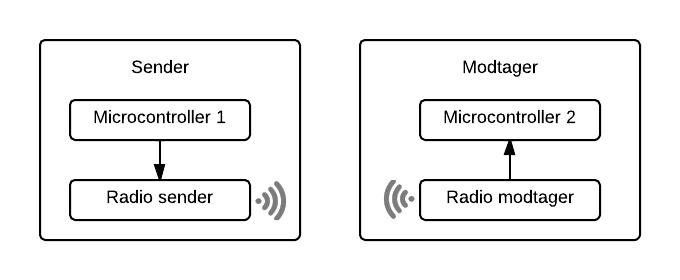
\includegraphics[scale=0.6]{Blokdiagram}
\caption{Skitse af hardware}
\end{figure}

\code{Senderen} er den brugeren laver sit indput på. 
\\ \code{Modtageren} er den enhed der er sat på dronen, som skal modtage signalet fra senderen.\\
Det vil sige der skulle laves to enheder. Begge skulle gøre brug af chippen cc1101 fra texas instruments. Og microcontrolleren atmega8 fra Atmel Corporation.
\code{Senderen} skal også have knapper så brugeren kan lave sit indput.

\section{Grænseflader}

De interne og eksterne grænseflader. 

\subsection{Sender}
\begin{figure}[H]
\centering
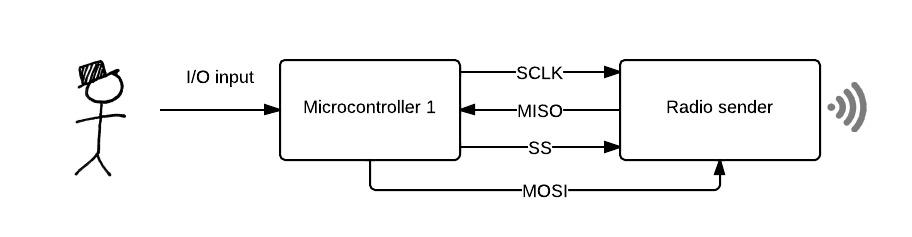
\includegraphics[scale=0.5]{SenderInterface}
\caption{Grænseflader for sender}
\label{fig: SenderInterface}
\end{figure}

På Figur \ref{fig: SenderInterface} ses et blokdiagram af senderen med alle grænseflader.


\subsection{Modtager}

\itoc

\section{Design}

\subsection{Strøm indput}

\section{PCB layout}



Opdeling i blokke.
Interface mellem blokkene, f.eks.:
Realisering af den enkelte blok
· Enhedstest af den enkelte blok

Analoge/digitale niveauer
o Impedanser,
o Protokol (f.eks. mellem PC og mikroprocessor)



\end{document}